\chapter{Intelligente Agenten in Videospielen}\label{intelligente_agenten}
\Fachbegriff{Intelligente Agenten} sind autonom handelnde Entitäten, deren Handlungen von bestimmten Zielen abhängen. Sie sammeln Beobachtungen aus einer simulierten oder realen Umgebung, auf deren Basis sie Entscheidungen treffen und die unter Umständen für einen Lernvorgang genutzt werden können. Oft wird dabei auch von \ac{ai} bzw. \ac{ki} gesprochen. Intelligente Agenten werden häufig in Spielen verwendet, um unterschiedliche Arten von \Fachbegriff{Nicht-Spieler-Charakteren} (NPCs) zu simulieren. In der Spielwelt haben diese virtuellen Charaktere in der Regel eine visuelle Repräsentation, beispielsweise anhand einer Person oder eines Tieres, mit der der Spieler interagieren kann. Sie können sowohl eine neutrale Rolle einnehmen (Händler, Dorfbewohner), als auch eine dem Spieler gegenüber feindliche oder freundliche Gesinnung aufweisen (Gegner, Gefährte).

Es gibt eine Vielzahl von Technologien die für die Entscheidungsfindung intelligenter Agenten genutzt werden können. Sowohl die Wahl des Verfahrens als auch der aufgebrachte Aufwand spielen eine kritische Rolle für die Authentizität und die erreichte Intelligenz des Agenten. Im Laufe der Jahre haben diese fortwährend an Komplexität gewonnen. Dabei wird der Versuch unternommen, biologische Verhaltensmuster nachzuahmen, um eine Art von pseudo-intelligentem Verhalten zu erschaffen. Die Definition von \textit{Intelligenz} oder \Fachbegriff{künstlicher Intelligenz} ist dabei allerdings unpräzise, da es keine allgemeingültige Definition gibt.

Nach Russel und Norvig \cite{art_int_mod_app} könnte bereits eine simple Maschine wie ein Thermostat als intelligenter Agent bezeichnet werden, da er eigenständig auf äußere Einflüsse reagiert. Laut dieser Definition könnten auch Software-Agenten wie Mining-Bots, die scheinbar eigenständig Daten sammeln, als intelligente Agenten bezeichnet werden. Nikola Kasabov \cite{kasabov} bietet hingegen eine vollkommen andere  Definition intelligenter Agenten anhand einer Menge von Anforderungen an den Agenten:

\begin{itemize}
    \item Regeln für Problemlösungen müssen inkrementell angepasst werden.
    \item Die Anpassung muss in Echtzeit stattfinden.
    \item Eine Selbstanalyse bezüglich des Verhaltens und des Erfolgs muss stattfinden.
    \item Ein Lernvorgang durch Interaktion mit der Umgebung muss gegeben sein.
    \item Der Lernvorgang muss mit einer ausreichenden Datenmenge schnell ablaufen.
    \item Es muss ein Gedächtnis vorhanden sein.
    \item Parameter für die Realisierung von Kurz- und Langzeitgedächtnis sowie das Vergessen von Erinnerungen müssen gegeben sein.
\end{itemize}

Kein intelligenter Agent in einem Spiel ist bisher in der Lage, diesen Anforderungen gerecht zu werden. Alternative Definitionen gehen in der Regel nicht über die Anforderung hinaus, dass der Agent selbst handeln muss.

Der Begriff \Fachbegriff{Intelligenter Agent} wird daher im Folgenden stets als Software-Agent in Umfeld einer simulierten Realität anhand von Videospielen definiert, der selbst Entscheidungen trifft. Ziel dieses Agenten ist eine sinnvolle Entscheidungsfindung zwecks einer Interaktion mit dem Spieler. Dabei soll so weit wie möglich eine scheinbare Imitation menschlichen Verhaltens umgesetzt werden, es werden allerdings keine weiteren Anforderungen an Lernvorgänge oder ein Gedächtnis gestellt. Dafür kann eine analytische, formale Vorgehensweise der Verfahren für die Entwicklung von Algorithmen für Agenten verwendet werden. Alternativ wird der Versuch unternommen, biologische oder kognitive Prozesse zu imitieren, um intelligentes Verhalten zu simulieren. Unabhängig von der gewählten Technologie soll lediglich der Eindruck von Intelligenz erweckt werden, ohne dass dabei tatsächliche Intelligenz erreicht werden muss. Die von Kasabov definierten Kriterien bezüglich eines Lernvorgangs oder einem Gedächtnisvermögen etc. sind daher nur optionale Eigenschaften.
Im folgenden Abschnitt werden einige etablierte Methoden für die Entscheidungsfindung intelligenter Agenten vorgestellt.


\section{Finite State Machines}
Bei \Fachbegriff{Finite State Machines} oder \Fachbegriff{Endlichen Automaten} handelt es sich um abstrakte Zustandsmaschinen, die sich in jeweils einem von mehreren Zuständen befinden können \cite{ai_for_game_devs} \cite{rich_basic_game_ai_course} \cite{cmsc_425} \cite{state_machine_flora_game} \cite{game_ai_by_example}. Das Ziel des Verfahrens ist eine reduzierte Abbildung der Wirklichkeit anhand eines Modells, welches durch die State Machine beschrieben wird. Die State Machine stellt also nur den Ansatz einer Simulation der Wirklichkeit dar, sowie auch alle weiteren vorgestellten Technologien für intelligente Agenten. Dafür müssen Zustände und Zustandsübergänge bzw. \Fachbegriff{States} und \Fachbegriff{Transitions} definiert werden. Die Zustandsübergänge schaffen Verbindungen in andere Zustände und werden durch bestimmte Konditionen gestartet, sogenannte \Fachbegriff{Trigger}. Ein populäres Beispiel für Spiele, in denen State Machines zum Einsatz kommen, ist das 1992 veröffentliche \Fachbegriff{Wolfenstein 3D} \cite{wolfenstein}.

\begin{figure}[H]
\centering
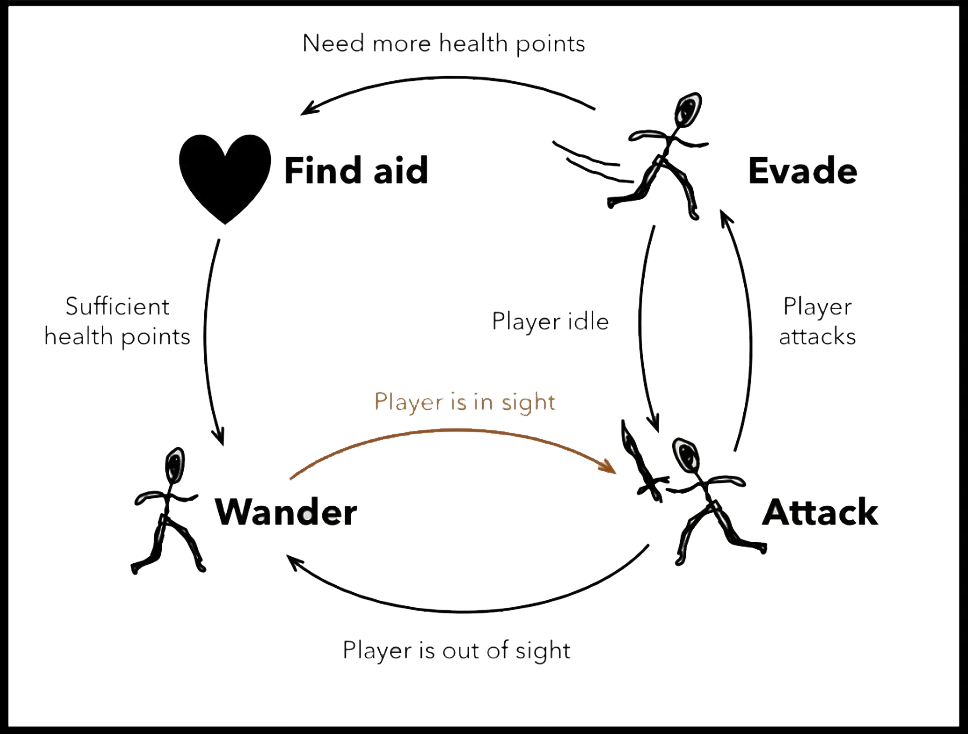
\includegraphics[scale=0.3]{images/chapter_2_int_agents/state_machine.png}
\caption{Beispielhafte Finite State Machine \cite{art_int_vid_games_towardsdatascience}}
\label{fig:state_machine_1}
\end{figure}

Die Abbildung \ref{fig:state_machine_1} zeigt eine Finite Sate Machine anhand eines simplifizierten Beispiels. Es werden die Zustände \aufzaehlung{Find aid}, \aufzaehlung{Wander}, \aufzaehlung{Attack} und \aufzaehlung{Evade} für einen NPC definiert. Wenn der NPC sich im \textit{Wander}-Zustand befindet, so kann er lediglich in den \textit{Attack}-Zustand wechseln. Der Trigger dafür ist die Sichtbarkeit des Spielers. Sobald die Triggerkondition eintrifft, findet ein Zustandsübergang in den \textit{Attack}-Zustand statt. Für diesen Zustand gibt es nun zwei mögliche Zustandsübergänge: Wenn der Spieler ebenfalls angreift, so wechselt der NPC in den \textit{Evade}-Zustand und versucht, vor dem Spieler zu flüchten. Wenn der Spieler außer Sicht ist, wechselt er zurück in den \textit{Wander}-Zustand. Aus dem \textit{Evade}-Zustand heraus kann der NPC zurück in den \textit{Attack}-Zustand wechseln, wenn der Spieler sich im \Fachbegriff{Idle}-Modus befindet, also nichts tut. Weiterhin wechselt der NPC in den \textit{Find Aid}-Zustand, sobald seine Lebenspunkte unter einem bestimmten Wert liegen. Wenn seine Lebenspunkte aufgefüllt wurden findet ein Zustandsübergang in den \textit{Wander}-Zustand statt.

Die folgenden Codebeispiele (siehe Listings \ref{lst:fsm_state} bis \ref{lst:fsm_getactions}) zeigen eine mögliche minimalistische Implementierung der State Machine: 

\begin{tabular}{ll}
\begin{minipage}{.48\textwidth}
\begin{lstlisting}[linewidth=7.25cm, label=lst:fsm_state, caption=State Class, xleftmargin=1.9cm]
class State {
    var action;
    var entryAction;
    var exitAction;
    var transitions;
}
\end{lstlisting}
\end{minipage}
\hfill

\begin{minipage}{.48\textwidth}
\begin{lstlisting}[linewidth=7.25cm, label=lst:fsm_transition, caption=Transition Class, xleftmargin=1.7cm]
class Transition {
    var state;
    function isActive;
}
\end{lstlisting}
\end{minipage}
\end{tabular}

\begin{minipage}{\linewidth}
\begin{lstlisting}[linewidth=16.4cm, label=lst:fsm_example-state, caption=Beispiel-State, xleftmargin=1cm]
class AttackState extends State {
  var action = new AttackAction();
  var entryAction = new MoveAndDrawSwordAction();
  var exitAction = new SheathSwordAction();
  var transitions = [new WanderAttackTransition(),
    new EvadeAttackTransition()];
}
\end{lstlisting}
\end{minipage}

\begin{minipage}{\linewidth}
\begin{lstlisting}[linewidth=16.4cm, label=lst:fsm_example-transition, caption=Beispiel-Transition, xleftmargin=1cm]
class WanderAttackTransition extends Transition {
  var state = new AttackState();
  function isActive() {
    return isPlayerClose();
  }
}
\end{lstlisting}
\end{minipage}

\begin{minipage}{\linewidth}
\hspace{2cm} \begin{lstlisting}[linewidth=16.4cm, label=lst:fsm_getactions, caption=State Machine Controller, xleftmargin=1cm]
class StateController {
    [...]

    function getActions() {
        activeTransition = null;
        foreach (transition in currentState.transitions) {
            if (transition.isActive()) {
                activeTransition = transition;
                break;
            }
        }
        if (activeTransition != null) {
            newState = activeTransition.state;
            actions += currentState.exitAction;
            actions += newState.entryAction;
            actions += newState.action;
            currentState = newState;
            return actions;
        } else return [currentState.action];
    }
}
\end{lstlisting}
\end{minipage}

Zunächst werden die Klassen \inlinecode{State} und \inlinecode{Transition} definiert. \inlinecode{State} benötigt die ausführbare Hauptaktion \inlinecode{action}, sowie eine Eingangs- und Ausgangsaktion, wie beispielsweise eine bestimmte Animation, die für einen flüssigen Übergang der Zustände ausgeführt wird. Für den Zustand \inlinecode{AttackState} werden daher entsprechende Aktionen für das Aufnehmen sowie Verstauen eines Schwertes definiert. Die Hauptaktion \inlinecode{AttackAction} sorgt dafür, dass eine Attacke ausgeführt wird. Weiterhin werden zwei Zustandsübergänge \inlinecode{WanderAttackTransition} und \inlinecode{EvadeAttackTransition} definiert, da der \ac{npc} entweder aus dem \Fachbegriff{Wander}- oder aus dem \Fachbegriff{Evade}-Zustand in den \Fachbegriff{Attack}-Zustand wechseln kann.
Jede Transition verfügt dabei über den Zielzustand und über eine Funktion \texttt{isActive}, die angibt, ob die Transition aktiv ist. Die \texttt{WanderAttackTransition} definiert daher \texttt{AttackState} als Zielzustand und prüft innerhalb von \texttt{isActive}, ob ein Spieler in der Nähe ist.
Der \texttt{StateController} prüft nun mittels der Funktion \texttt{getActions} in regelmäßigen Abständen oder nach dem Ausführen von Einzelaktionen durch das Aufrufen der \texttt{isActive}-Funktionen für alle Transitions, ob neue Zustandsübergänge verfügbar sind. Sobald eine solche gefunden wird, wird der neue Zustand gesetzt und sowohl die Ausgangsaktion des aktuellen Zustands, sowie die Eingangs- und die Hauptaktion des neuen Zustands werden in die Liste der auszuführenden Aktionen aufgenommen. Ansonsten wird stets die Hauptaktion des aktuellen Zustands weiterhin ausgeführt.

Nach diesem einfachen Schema werden Zustände und ihre Übergänge definiert. Der \Fachbegriff{StateController} stellt anschließend sicher, dass Zustandsübergänge automatisch eingeleitet werden. In diesem Beispiel wird immer der erste mögliche Zustandsübergang genommen, theoretisch könnte man den Übergängen nun aber Prioritäten zuweisen. Die Architektur und das Anlegen neuer Zustände sind simpel und effizient. Bei der Darstellung aller möglichen Zustände eines echten, komplexen Spiels werden jedoch schnell Grenzen erreicht, da eine hohe Menge von Zuständen und Übergängen erreicht wird. Aufgrund des hohen Determinismus von State Machines in ihrere einfachen Form eignen sie sich weiterhin nicht für den Einsatz in jedem Spiel. Man stelle sich ein Strategiespiel vor, in dem State Machines für NPC-Gegner verwendet werden. Diese Gegner würden jedes Mal auf die gleiche Art und Weise auf bestimmte Situationen reagieren. Das ist zum einen problematisch, weil dadurch statt einem authentischen, dynamischen Verhalten lediglich eine repetitive Spielerfahrung zustandekommt und zum anderen, weil derartiges Verhalten vorhersehbar ist und daher leicht durch den Spieler ausgenutzt werden kann.


\paragraph{Hierarchical State Machines}
% https://www.cs.umd.edu/class/spring2019/cmsc425/handouts/lect21-ai-dec-making.pdf
State Machines haben zusätzlich das Problem, dass die Anzahl der Zustände schnell große und daher unübersichtliche Ausmaße annehmen kann. Außerdem ist es nur möglich, einen einzelnen Zustand zur Zeit einzunehmen, wodurch nur sehr eingeschränktes Verhalten realisiert werden kann. Möchte man beispielsweise modellieren, dass ein NPC zur selben Zeit verwundet ist und gleichzeitig den Spieler angreift, muss dafür ein eigener neuer Zustand \Fachbegriff{IsAttackingWhileWounded} entworfen werden. Wenn man erreichen will, dass der Spieler in jedem bereits entworfenen Zustand ebenfalls verwundet sein kann, muss dann eine Vielzahl neuer Zustände entworfen werden. So resultiert die Kombination aus allen möglichen Zuständen für die Erstellung neuer Sub-Zustände und Sub-Transitions oft in vollkommen unbrauchbaren Zustandsmengen, die nicht mehr verwaltet werden können.

Eine mögliche Lösung für diese Probleme ist die Entwicklung von State Machines in einer hierarchischen Struktur. Dafür gibt es eine Anzahl von \Fachbegriff{High-Level}-Zuständen, die einen allgemeinen, übergeordneten Kontext für das Charakterverhalten darstellen. In jedem dieser High-Level-Zuständen gibt es dann mehrere \Fachbegriff{Sub-Level}-Zustände, die für spezifischeres Verhalten sorgen. Solche Systeme werden als \Fachbegriff{Hierarchical State Machines} bezeichnet \cite{cmsc_425}. Die Struktur des Verfahrens lässt gewisse Gemeinsamkeiten zu UML-Diagrammen erkennen, in denen ebenfalls hierarchisch geschachtelte Gruppen von Aktionen gebildet werden.

Als weiteres Beispiel wird ein Agent angeführt, der die Zustände \aufzaehlung{On Guard}, \aufzaehlung{Fight} und \aufzaehlung{Run Away} mit Transitions untereinander besitzt. Jetzt soll ein neuer Zustand \aufzaehlung{Get Food} eingeführt werden, der zu jeder Situation eintreten kann, sobald der Agent hungrig ist. Von jedem möglichen Zustand müsste dann ein Übergang zu dem neuen Zustand geschaffen werden (siehe Abbildung \ref{fig:hierchical_state_machine_bot_1}).

\begin{figure}[H]
\centering
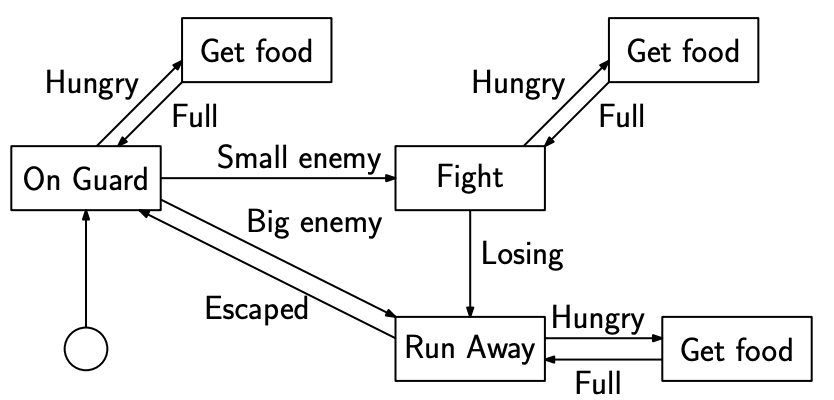
\includegraphics[scale=0.74]{images/chapter_2_int_agents/hierarchical_state_machine_1_without.png}
\caption{Hinzufügen eines neues Zustands, normale State Machine}
\label{fig:hierchical_state_machine_bot_1}
\end{figure}

\begin{figure}[H]
\centering
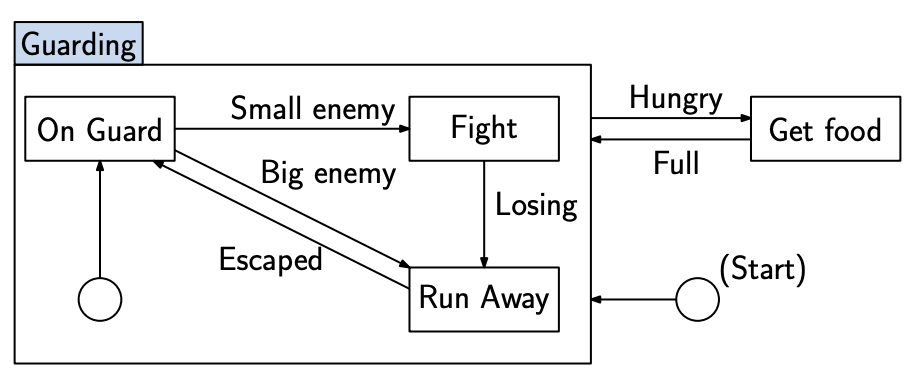
\includegraphics[scale=0.7]{images/chapter_2_int_agents/hierarchical_state_machine_2_with.png}
\caption{Hinzufügen eines neues Zustands, hierarchische State Machine}
\label{fig:hierchical_state_machine_bot_2}
\end{figure}

Abbildung \ref{fig:hierchical_state_machine_bot_2} zeigt den gleichen Vorgang des Ergänzens um einen weiteren Zustand mit einer hierarchischen State Machine, statt einer herkömmlichen. Es wird ein neuer High-Level-State \Fachbegriff{Guarding} gebildet, der die bereits vorhandenen Zustände enthält. Dieser neue \sogenannt{Super-State} verfügt nun über einen Startpunkt, der nur dann angesprochen wird, wenn man das erste mal den Super-State betritt. Die Zustandsübergänge von jedem Sub-Zustand des Super-States sind implizit gegeben. Das könnte beispielsweise funktionieren, indem ein Stack verwendet wird, der die aktiven Zustände nach ihren Level sortiert, sodass der Zustand mit dem höchsten Level immer an der ersten Stelle des Stacks steht. Um mögliche Transitions zu prüfen, würde dann vom letzten bis zum ersten Element geprüft werden, ob ein Zustand für die bestimmte Aktion verfügbar ist \cite{cmsc_425}.

Die Architektur der State Machine wird dadurch simplifiziert und modularisiert, da insgesamt deutlich weniger Zustände verwaltet und erzeugt werden müssen. Weiterhin können insgesamt mehr Zustände verarbeitet werden, weil die Transitions vieler Zustände automatisch implizit definiert werden.



\section{Decision Trees}
% unreal tournament 2004: https://www.researchgate.net/publication/221308927_Decision_Tree-Based_Algorithms_for_Implementing_Bot_AI_in_UT2004
Ein klassisches Verfahren für die Entscheidungsfindung intelligenter Agenten beruht auf der Verwendung von \Fachbegriff{Decision Trees}. Dabei wird eine einfache Baumstruktur aus möglichen Entscheidungen gebildet. Genauer handelt es sich um einen gewurzelten Baum. Häufig findet man binäre Bäume vor. Das Verfahren ist besonders sinnvoll, wenn der Agent aus vielen mögliche Entscheidungen zur selben Zeit auswählen muss. Je nachdem welche Entscheidung gewählt wurde, öffnet sich ein neuer Zweig des Baumes, unter Umständen mit weiteren Entscheidungen und möglichen Abstiegen.
Die Knoten des Baumes werden als \sogenannt{Decision Point}, also \Fachbegriff{Entscheidungsknoten}, bezeichnet. Jeder Entscheidungsknoten prüft eine bestimmte binäre Bedingung, beispielsweise: \textit{Ist der Spieler sichtbar?}. Damit wird eine Bedingung für den Abstieg des Baumes aufgestellt. Die Antwort auf die Bedingung ist dafür verantwortlich, ob ein Abstieg in den linken oder rechten Zweig des Entscheidungsknotens erfolgt. Bei einem binären Baum handelt es sich um \sogenannt{Ja-oder-Nein}-Fragen. Abbildung \ref{fig:decision_tree_1} zeigt ein Beispiel für einen typischen, stark simplifizierten Entscheidungsbaum für einen kämpfenden NPC.

\begin{figure}[H]
\centering
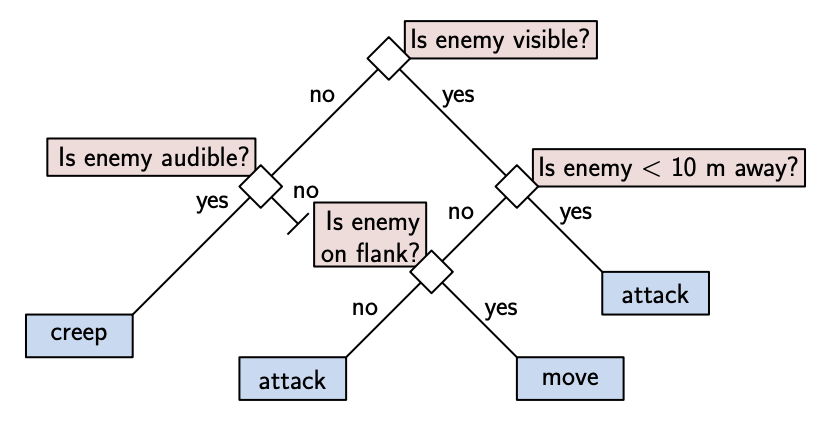
\includegraphics[scale=0.85]{images/chapter_2_int_agents/decision_tree_example_1.png}
\caption{Beispielhafter Decision Tree \cite{cmsc_425}}
\label{fig:decision_tree_1}
\end{figure}

% beispiele? besonderheiten?
% man könnte heir die erweiterten bäume mit aufnehmen..
% https://www.cs.umd.edu/class/spring2019/cmsc425/handouts/lect21-ai-dec-making.pdf


Decision Trees sind einfach zu verstehen und können leicht implementiert werden. Zusätzlich bieten sie eine hohe Performanz. Neben der Entscheidungsfindung von NPCs haben sie noch weitere Anwendungsbereiche in Videospielen. Beispielsweise werden Bäume für Questsysteme eingesetzt. Das Spiel \Fachbegriff{Witcher 3} \cite{witcher_3} verwendet beispielsweise Decision Trees, um je nach den Handlungen des Spielers im Spiel den Ablauf vom Ende des Spiels festzulegen.

% Monte Carlo search trees
% https://towardsdatascience.com/artificial-intelligence-in-video-games-3e2566d59c22



\section{Behavior Trees}
\Fachbegriff{Behavior Trees} sind eine Weiterentwicklung von Finite State Machines, bei der Baumstrukturen genutzt werden. Sie gehen von einem modularen komponentenbasierten System für das Verhalten bzw. \textit{Behavior} von Agenten aus und verwendet dafür gewurzelte Bäume \cite{cmsc_425} \cite{ai_for_game_devs} \cite{gamasutra_behavior_tree}. Der erste Einsatz von Behavior Trees erfolgte im Jahr 2004 im erfolgreichen Spiel \Fachbegriff{Halo 2} \cite{halo_behavior_tree_gdc} \cite{halo_2}.
Ein beispielhafter Behavior Tree ist in Abbildung \ref{fig:behavior_tree_1} zu sehen.

\begin{figure}[H]
\centering
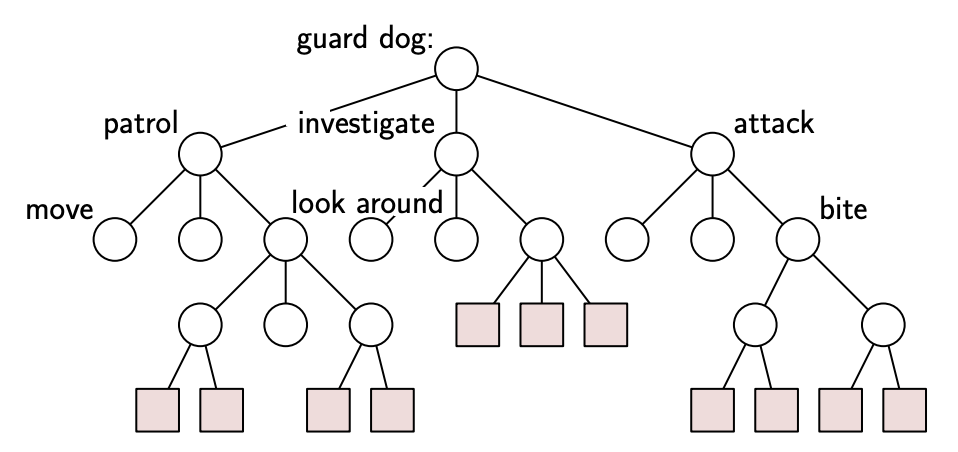
\includegraphics[scale=0.8]{images/chapter_2_int_agents/behavior_tree_1.png}
\caption{Beispielhafter Behavior Tree \cite{cmsc_425}}
\label{fig:behavior_tree_1}
\end{figure}

Die Knotenpunkte des Baumes enthalten sogenannte \Fachbegriff{Tasks} - spezifische Aufgaben, die ein explizites Ziel verfolgen. Tasks besteht aus einer Menge von Konditionen die bestimmen, welcher Task aktiv ist, sowie Aktionen, die die Ausführung des Tasks enkodieren. Da Tasks fehlschlagen können, geben diese bei der Ausführung einen von drei Statusberichten an: \textit{Running}, \textit{Success} oder \textit{Failure}. Alle im Baum enthaltenen Tasks sind Akteuren des Spiels zugewiesen. Die Granularität der Tasks erhöht sich mit steigender Tiefe des Baumes. Jeder Task beschreibt dabei ein Sub-Verhalten, das eine bestimmte Aufgabe im Kontext des übergeordneten Knotens übernimmt. Die Wurzel des Baumes beschreibt das generelle Verhalten für eine bestimmte Entität. Sie könnte beispielsweise das Verhalten \Fachbegriff{Gegner} oder \Fachbegriff{Wachhund} darstellen. 
Einzelne Top-Level-Tasks (Knoten direkt unter der Wurzel) beschreiben allgemeines Verhalten, wie beispielsweise \aufzaehlung{Angreifen}, \aufzaehlung{Umschauen} oder \aufzaehlung{Patroullieren}. Die Sub-Tasks von \textit{Angreifen} könnten zum Beispiel \textit{Schlagen} oder \textit{Schießen} sein.

Die Blätter des Baumes beschreiben die tatsächliche Interaktion der Entität mit dem Spiel und die Ausführung von Aktionen. Sie beinhalten Konditionen, die erfüllt sein müssen, und Aktionen, die dann ausgeführt werden. Für das Beispiel des Wachhundes könnten die Konditionen den Zustand des Hundes (\textit{Ist der Hund hungrig? Ist der Hund verletzt?}) oder den allgemeinen Spielzustand betreffen (\textit{Ist ein Gegner in der Nähe?}). Die mit den Konditionen verbundenen Aktionen verändern dann dessen Zustand - der Hund könnte beispielsweise den Spieler beißen und seine Lebenspunkte verringern oder einfach eine Animation abspielen. Die Konditionen können auch als Filter betrachtet werden, die bestimmen, welche Aktionen ausgeführt werden\cite{cmsc_425}.


\paragraph{Task Composition}
Behavior Trees bieten verschiedene Möglichkeiten für die Komposition von Tasks. Typischerweise werden Tasks entweder sequentiell oder ausgewählt abgearbeitet.

Bei der sequentiellen Ausführung von Tasks wird eine Liste von Tasks nacheinander verarbeitet (\Fachbegriff{Sequences}). Sobald ein Task fehlschlägt, wird die Sequenz terminiert. Eine beispielhafte Ausführung wird anhand der Abbildung \ref{fig:behavior_tree_2} verdeutlicht. Der Pfeil in der Grafik steht für die sequenzielle Ausführung der Aktionen.

\begin{figure}[H]
\centering
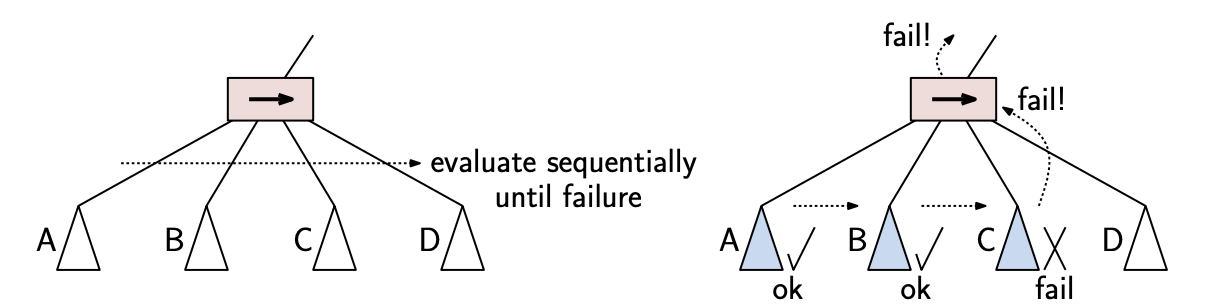
\includegraphics[scale=0.75]{images/chapter_2_int_agents/behavior_tree_2.png}
\caption{Sequenzielle Ausführung in Behavior Tree \cite{cmsc_425}}
\label{fig:behavior_tree_2}
\end{figure}

Bei der ausgewählten Ausführung (\Fachbegriff{Selector}) wird maximal ein Task aus einer Menge von Tasks ausgewählt. Sobald der erste Task einen erfolgreiche Statusbericht versendet, wird die Ausführung terminiert. Abbildung \ref{fig:behavior_tree_3} zeigt eine beispielhafte ausgewählte Ausführung. Das Fragezeichen verdeutlicht in der Abbildung den Selector, eine ausgewählte Ausführung bis zum ersten Erfolg.

\begin{figure}[H]
\centering
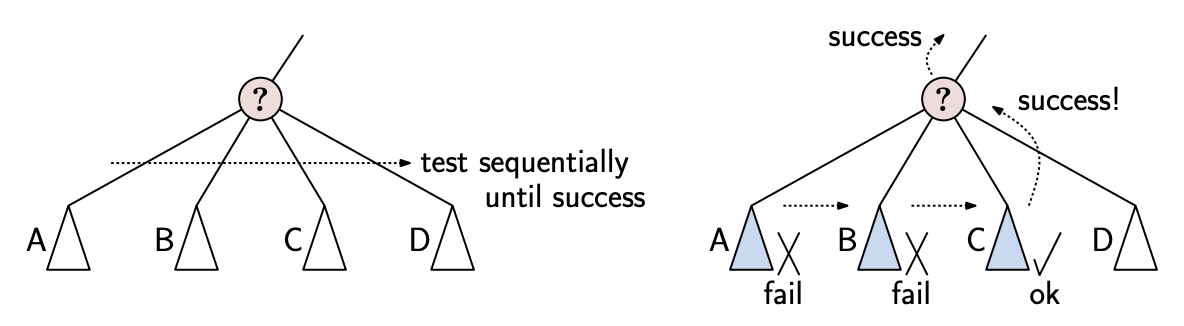
\includegraphics[scale=0.75]{images/chapter_2_int_agents/behavior_tree_3.png}
\caption{Ausgewählte Ausführung in Behavior Tree \cite{cmsc_425}}
\label{fig:behavior_tree_3}
\end{figure}

Mit Sequences und Selector werden den Behavior Trees einige Möglichkeiten hinzugefügt, die für Finite State Machines nicht verfügbar sind. Sequences und Selector können kombiniert werden, um ein komplexeres Verhalten zu realisieren. Einzelne Teilbäume dieses Verhaltens können dann auf Sequences und andere Teilbäume auf Selector basieren.
In Abbildung \ref{fig:behavior_tree_4} ist ein konkretes Beispiel für eine Kombination von Selector und Sequence zu erkennen, in dem ein NPC auf verschiedene Art und Weise je nach Beschaffenheit des Spielzustands versucht, in einen Raum zu gelangen. Anhand der Symbole in der Grafik (\sogenannt{!} und \sogenannt{?}) ist die Kombination von Selector und Sequence erkennbar. Der Agent betritt unmittelbar den Raum, wenn die Tür offen ist. Falls dies nicht gelungen ist, bewegt er sich zunächst zur Tür und versucht anschließend, diese zu öffnen. Wenn auch dies scheitert, wird die Tür aufgebrochen, sodass der Agent schlussendlich den Raum betreten kann.

\begin{figure}[H]
\centering
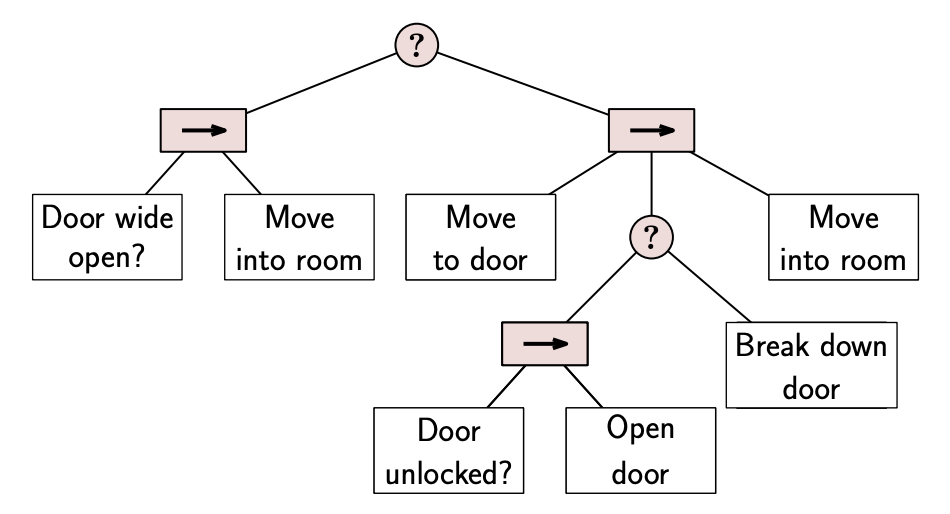
\includegraphics[scale=0.75]{images/chapter_2_int_agents/behavior_tree_4.png}
\caption{Kombination sequenzieller und ausgewählter Ausführung in Behavior Tree \cite{cmsc_425}}
\label{fig:behavior_tree_4}
\end{figure}

Aus der Sicht des Software-Engineering werden dem Programmierer mit Behavior Trees ein besser strukturierter Kontext für die Entwicklung von Verhalten zur Verfügung gestellt \cite{cmsc_425}. Da sie alle Vorteile von Finite State Machines bieten und darüber hinaus über eine hohe Performanz verfügen, sind Behavior Trees zu einer sinnvollen Alternative zu State Machines geworden \cite{behavior_tree_article}. Sie werden daher zunehmend in großem Maßstab in erfolgreichen und komplexen Spielen wie \Fachbegriff{Halo}, \Fachbegriff{Bioshock} oder \Fachbegriff{Spore} verwendet \cite{behavior_tree_wiki}.




\section{Goal Oriented Action Planning (GOAP)}\label{goap}
\ac{goap} ist ein System für die Planung und Ausführung von Aktionen für einen Agenten und wurde zunächst für das Spiel \Fachbegriff{F.E.A.R.} entwickelt \cite{goap_fear}. Es erlaubt einem Agenten die Planung einer Sequenz von Aktionen zum Erreichen eines bestimmten Ziels. GOAP bietet gegenüber Finite State Machines den Vorteil, dass keine großen Mengen von Zuständen und Zustandsübergängen definiert werden müssen \cite{goap_gamedevelopment} \cite{game_ai_by_example}. Anstelle von Zuständen werden hier modulare, voneinander entkoppelte Aktionen verwendet \cite{goap_haw}.

GOAP verlangt für die Entscheidungsfindung lediglich die Definition von \Fachbegriff{Goals} und \Fachbegriff{Aktionen} \cite{ai_for_game_devs}. Goals sind festgelegte Konditionen, die ein Agent erfüllen möchte. Um ein Goal zu erreichen, werden Aktionen ausgeführt, die den Spielzustand verändern. Eine Kette aus Aktionen wird aufgebaut, die den Spielzustand so verändern, dass die Konditionen des Goals erfüllt sind. Bei einer Aktion kann es sich beispielsweise um das simple Öffnen einer Tür oder das Aufnehmen eines Gegenstands in das Inventar des NPCs handeln. Die vom Agenten ausgeführten Aktionen haben jeweils eine Menge von Bedingungen (\Fachbegriff{Preconditions}), die für die Ausführung der Aktion vorausgesetzt werden, sowie eine Menge von Effekten als eine Folge der Aktion. Diese sorgen dafür, dass die Bedingung eines Goals schlussendlich erfüllt wird.

Aus den einzelnen Aktionen erstellt der sogenannte \Fachbegriff{GOAP Planner} eine Sequenz zum Erreichen eines Ziels. Es handelt sich um eine zentrale Verwaltungs- und Planungseinheit für die Ausführung von Aktionen im GOAP-System. Der GOAP Planner kennt die Bedingungen der Goals sowie die Preconditions und Effekte der Aktionen. Auf dieser Grundlage ist er in der Lage zu erkennen, welche Effekte welcher Aktionen benötigt werden, um das Goal zu erreichen. Dadurch kennt der GOAP Planner auch die Preconditions der benötigten Aktionen und kümmert sich ebenfalls darum, dass diese Bedingungen erfüllt werden. Dafür werden unter Umständen weitere Aktionen in die Sequenz eingefügt. Der Planner stellt sicher, dass die benötigten Ketten von Aktionen in der richtigen Reihenfolge ausgeführt werden.
Konkret sucht der GOAP Planner zunächst nach allen vorhandenen Goals. Für diese erstellt er rückwärts vom Goal aus gehend eine Baumstruktur. Diese besteht aus allen möglichen Sequenzen von Aktionen, die zum jeweiligen Ziel führen. Dabei wird der jeweils kürzeste Weg gewählt, der zum Ziel führt. Die Pläne des Agenten sind nicht statisch, sondern werden erst zur Laufzeit generiert, sodass dieser sich dynamisch an die jeweiligen Umstände seiner Umgebung anpassen kann. In der Abbildung \ref{fig:goap_1} ist eine beispielhafte Sequenz in einem GOAP-System zu erkennen.

\begin{figure}[H]
\centering
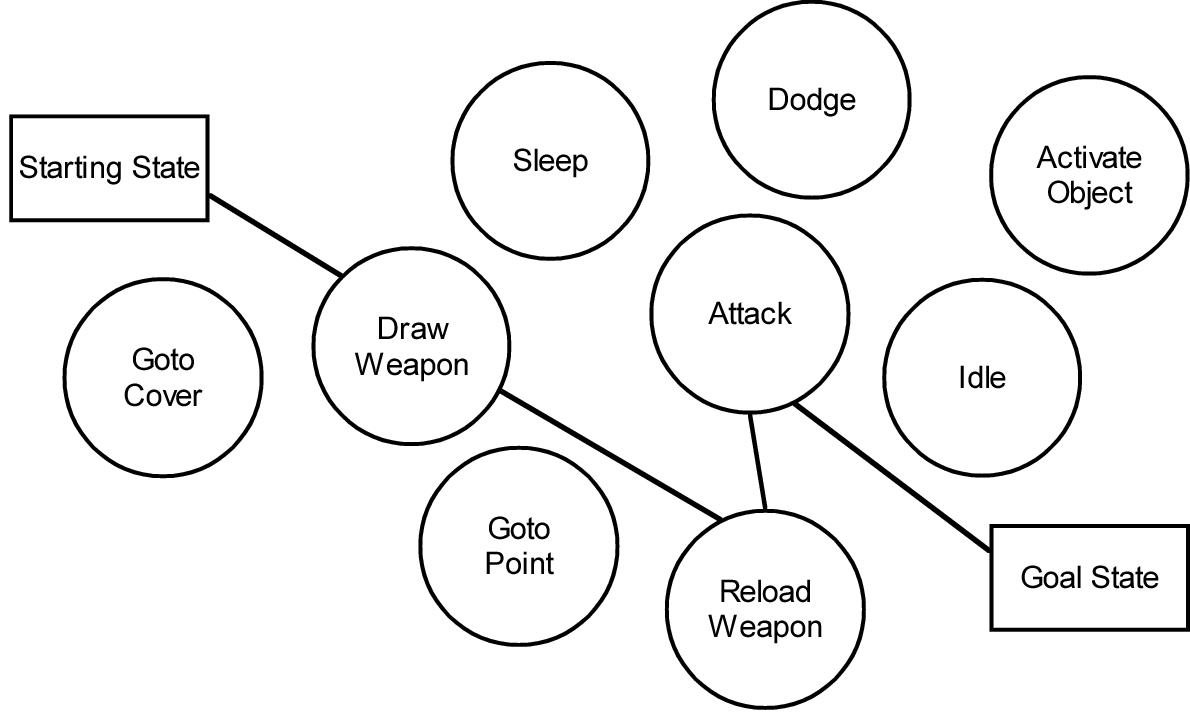
\includegraphics[scale=0.25]{images/chapter_2_int_agents/goap_1.png}
\caption{GOAP-Sequenz nach Orkin \cite{goap_fear}}
\label{fig:goap_1}
\end{figure}

Es sei darauf geachtet, dass keine Übergänge zwischen den Aktionen vorhanden sind. Die Abbildung zeigt das GOAP-Äquivalent einer State Machine mit übergangslosen Aktionen statt Zuständen und Transitions.
Intern verwendet GOAP eine minimale State Machine, die über drei Zustände verfügt: \aufzaehlung{Idle}, \aufzaehlung{MoveTo} und \aufzaehlung{PerformAction}. Das ist notwendig, da sich der Agent für einige Aktionen in der Nähe eines bestimmten Objekts befinden muss. Das Bewegen des Agenten ist nicht Teil des eigentlichen GOAPs, weil sonst viele zusätzliche Aktionen für die Bewegung zu bestimmten Zielen von Aktionen definiert werden müssten. Stattdessen kann jeder Aktion bei Bedarf ein Ziel zugewiesen werden.
Im \Fachbegriff{Idle}-Zustand hat der Agent eine vorherige Sequenz von Aktionen abgeschlossen. Der \Fachbegriff{GOAP Planner} berechnet nun die nächste Sequenz für das Erreichen eines Ziels. Der Agent wechselt dann in den \Fachbegriff{PerformAction}-Zustand. Vor dem Ausführen jeder Aktion wird geprüft, ob diese über eine Zielposition verfügt und ob der Agent sich nah genug an dieser Position befindet. Falls dies nicht der Fall ist, wechselt der Agent in den \Fachbegriff{MoveTo}-Zustand und anschließend wieder in den \Fachbegriff{PerformAction}-Zustand. In diesem Zustand führt der Agent eine GOAP-Aktion aus.

Die Vorteile von GOAP liegen in der Modularität des Systems. Das Hinzufügen und Austauschen von Aktionen ist ohne weiteres möglich. Der GOAP-Entwickler Orkin nennt ein Beispiel aus der Entwicklung von \Fachbegriff{F.E.A.R.}: Es wurde zum Ende der Entwicklungsphase die Bedingung gestellt, dass NPCs beim Betreten von Räumen stets das Licht anschalten sollen. Mit GOAP musste lediglich eine Aktion \Fachbegriff{TurnOnLightsAction} mit einem neuen Effekt \Fachbegriff{LightsOn} erstellt werden, der auch eine Precondition für die \Fachbegriff{GoToRoomAction} ist \cite{goap_fear}. Mit einer State Machine wäre dieser Vorgang komplexer gewesen und hätte deutlich mehr Zeit gekostet. Ein weiterer Vorteil ist, dass bei der Verwendung desselben Goals bei unterschiedlichen Agenten eine völlig unterschiedliche Sequenz von Aktionen erstellt werden kann, da diese vom Zustand des Spiels abhängen, sodass die Agenten dynamischer und realistischer wirken \cite{goap_gamedevelopment}.


\section{Utility Based Agents}\label{utility_agents}
\Fachbegriff{Utility Based Agents} beruhen auf einem AI-System namens \Fachbegriff{Utility-Based Action Bias}. Es basiert auf einer simplen Idee: Die Agenten wechseln nicht wie z.B. bei Finite States Machines zwischen einer endlichen Menge von Zuständen, die durch bestimmte Trigger ausgelöst werden, sondern bewerten kontinuierlich die ihnen zur Verfügung stehenden Aktionen basierend auf \Fachbegriff{Utility-Functions} $U(s_t)$ \cite{art_int_mod_app} \cite{utility_based_agents_2}. Diese Funktionen bestimmen, wie groß der daraus hervorgehende Vorteil für den Agenten ist - sie bestimmen also in gewisser Weise die \textit{Präferenzen} eines Agenten in Abhängigkeit von seinem Zustand $s_t$. Der Agent wählt stets die Aktion aus, die ihn in den Zustand mit dem höchsten Utility-Wert bringt. Die Effekte von Aktionen sind bekannt, sodass der Utility-Wert für einen neuen Zustand leicht berechnet werden kann.

In der \Fachbegriff{Utility Theory} wird davon ausgegangen, dass es eine Menge von Utility-Functions gibt, die nicht direkt mit Aktionen gekoppelt werden. In diesem Fall müssen alle möglichen neuen Zustände $s_{t+1}$ betrachtet werden, die aus den möglichen Aktionen $a$ aus der Menge aller Aktionen $\mathbb{A}$ hervorgehen. Da der Utility-Wert maximiert werden soll wird die Aktion $a$ ausgewählt, die den höchsten Wert $U(s_{t+1})$ erzielt, wie von Russel und Norvig beschrieben \cite{art_int_mod_app}:
$$ action = \argmax_a \: U(s_{t+1}) \:\;  \forall{a}	\in{\mathbb{A}} $$

Russell und Norvig unterscheiden weiterhin zwischen deterministischen und nichtdeterministischen Umgebungen des Agenten. Der Einfachheit halber wird diese Unterscheidung an dieser Stelle vernachlässigt, da sie in den meisten Fällen nicht relvant ist.
Wenn Utility-Based Agents in Spielen zum Einsatz kommen, werden Aktionen - anders als in der Literatur - meistens direkt mit ihrer eigenen Utility-Function gekoppelt. Jeder Aktion kann dann unmittelbar ein Utility-Wert zugewiesen werden, ohne dass zukünftige Zustände betrachtet werden. Man stelle sich beispielsweise eine Aktion vor, die die Waffe eines Agenten nachlädt. Die dazugehörige Utility-Funktion \sogenannt{Waffe nachladen} sinkt mit der Menge der Munition in der Waffe. Je niedriger der aktuelle Utility-Wert ist, desto höher ist der Utility-Gewinn beim Ausführen der Aktion.

Die Utility-Funktionen können vom Entwickler beliebig definiert werden, sodass sie dem Agenten ein dynamisches Verhalten verleihen. Beispielsweise könnte eine Utility-Funktion für die Benutzung eines Heiltranks so definiert werden, dass der Utility-Wert sich mit sinkender Anzahl der Lebenspunkte des Agenten erhöht. Somit steigt die Wahrscheinlichkeit für die Benutzung von Heiltränken mit sinkender Anzahl der Lebenspunkte, wie in Abbildung \ref{fig:utility_1} zu erkennen. Dafür wurde die Funktion $ f(x) = (1-(x/100))^4 $ verwendet.

\begin{figure}[H]
\centering
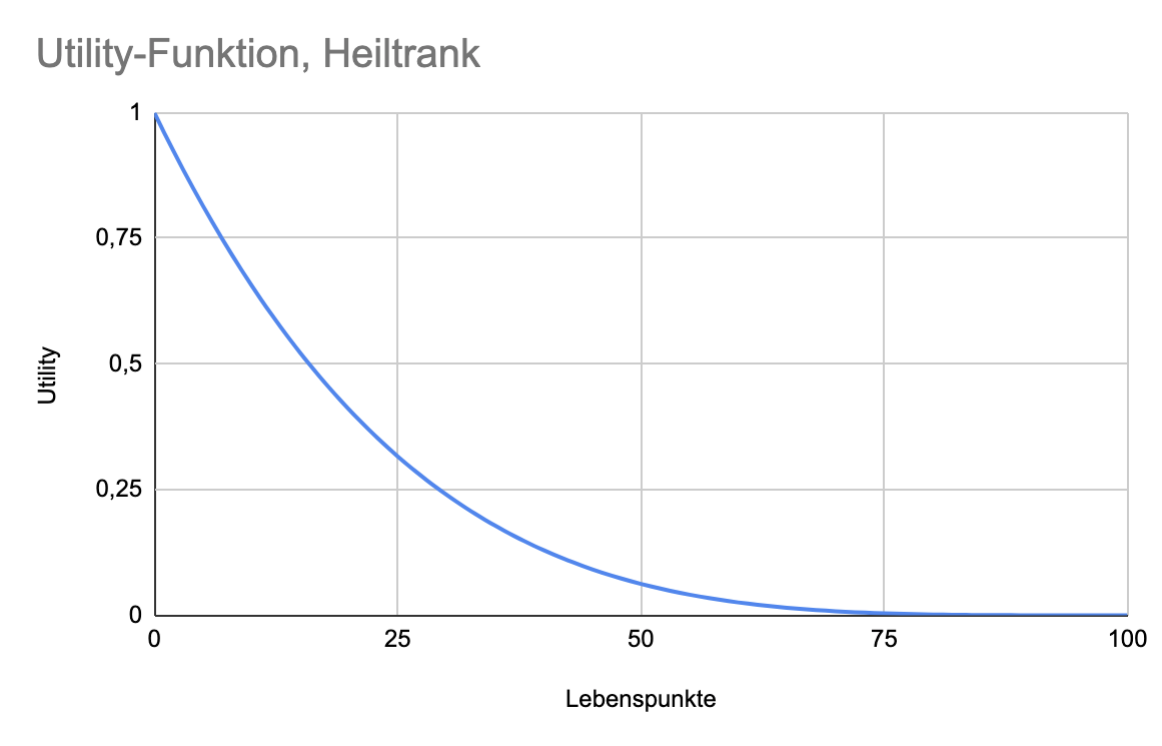
\includegraphics[scale=0.65]{images/chapter_2_int_agents/diagram_utility_1.png}
\caption{Utility-Funktion für Benutzung eines Heiltranks}
\label{fig:utility_1}
\end{figure}

Das Resultat der Verwendung von Utility-Funktionen für das Auslösen bzw. die Auswahl von Aktionen ist die Abbildung eines deutlich dynamischeren Verhaltens als beispielsweise bei der Verwendung einer Finite State Machine.

Eine Variante von Utility-Based Agents sind \Fachbegriff{Needs-Based Agents} \cite{needs_based_agents_1}. Die Utility-Funktionen in dieser Variante basieren auf indiviuellen Motivationen, die menschlichen Bedürfnissen nachempfunden wurden; beispielsweise \aufzaehlung{Hunger}, \aufzaehlung{Durst}, \aufzaehlung{Schlaf} oder \aufzaehlung{Kommunikation} \cite{needs_based_agents_1}. Damit soll ein möglichst menschliches Verhalten simuliert werden.

Mit dem Verfolgen von Bedürfnissen haben Utility-basierte Agenten nicht nur Wurzeln im Design von AI-Systemen, sondern mit der Utility Theory ebenfalls in der Psychologie und Soziologie \cite{utility_gdc}. Durch die beliebige Gestaltung von Bedürfnisfunktionen kann das Verhalten von Agenten verbessert werden. Besonders im Vergleich zu klassischen, statischen Methoden wie Finite State Machines kann daraus ein sinnvolleres, nachvollziehbares Entscheidungsverhalten resultieren. Ein populäres Beispiel für die Verwendung von Utility Based Agents (und in diesem Spezialfall Needs Based Agents) ist das Spiel \Fachbegriff{Die Sims 4} \cite{sims_4}. Das Spiel stellt eine Simulation von menschlichen Bedürfnissen und Beziehungen sowie des menschlichen Alltags dar. Es verwendet Utility-Funktionen für die Repräsentation des internen Zustands der NPCs, um ein annähernd menschliches Verhalten zu erreichen \cite{sims_utility}.









